\chapter[Declarative Scheduling in MapReduce]{Declarative Scheduling in MapReduce}
\label{ch:boom}

In this chapter, we turn to the problem of scheduling MapReduce tasks in the cloud. This work
is part of the \emph{BOOM} (Berkeley Orders of Magnitude) research
project, which aims to enable developers to build orders-of-magnitude more
scalable software using orders-of-magnitude less code than the state of the
art. The project is based on two hypotheses:
\begin{enumerate}
\item
  Distributed systems benefit substantially from a \emph{data-centric} design
  style that focuses the programmer's attention on carefully capturing all the
  important state of the system as a family of collections (sets, relations,
  streams, etc.)  Given such a model, the state of the system can be distributed
  naturally and flexibly across nodes via familiar mechanisms like partitioning
  and replication.
\item The key behaviors of such systems can be naturally implemented using
  \emph{declarative} programming languages that manipulate these collections,
abstracting the programmer from
  both the physical layout of the data and the fine-grained orchestration of
  data manipulation.
\end{enumerate}
Taken together, these hypotheses suggest that traditionally difficult
distributed programming tasks can be recast as data processing problems that are
easy to reason about in a distributed setting and expressible in a high-level
language.  In turn, this should provide significant reductions in code
complexity and development overhead, and improve system evolution and program
correctness.  We also conjecture that these hypotheses, taken separately, can
offer design guidelines useful in a wide variety of programming models.

In Section~\ref{ch:boom:sec:boom}, we present an overview of the BOOM project which
began with a reimplementation of the Hadoop architecture in the Overlog language. 
We then review some of the related work in Section~\ref{ch:boom:sec:relwork}.
Section~\ref{ch:boom:sec:jol} describes a new Java-based Overlog runtime that we use
to implement much of the Hadoop system functionality. We focus specifically on the
Hadoop MapReduce engine declarative port in this thesis, which is the topic of Section~\ref{ch:boom:sec:port}.
Finally, Section~\ref{ch:boom:sec:eval} presents an evaluation of our work.


\section{\BOOM}
\label{ch:boom:sec:boom}

The BOOM project began with an experiment in construction, by implementing a substantial piece of
distributed software in a data-centric, declarative style. Upon review of recent literature on
datacenter infrastructure (e.g.,~\cite{chubby,gfs-sosp,dynamo,mapreduce-osdi}),
we observed that most of the complexity in these systems relates to the
management of various forms of asynchronously-updated state, including sessions,
protocols, and storage. Although quite complex, few of these systems involve intricate, uninterrupted
sequences of computational steps. Hence, we suspected that datacenter
infrastructure might be a good initial litmus test for our hypotheses about building distributed software.

\emph{\BOOMA} is an API-compliant reimplementation of the HDFS distributed 
file system and the Hadoop MapReduce engine.  These two components were named \emph{\BOOM-FS} 
and \emph{\BOOM-MR}, respectively. In writing \BOOMA, we preserved the Java API ``skin'' of HDFS and 
Hadoop, but replaced complex internal state with a set of relations, and replaced key system logic with 
code written in a declarative language. This chapter focuses on the design of \BOOM-MR, which replaced 
the Hadoop task scheduling logic with a declarative scheduling framework. A description of \BOOM-FS can
be found in~\cite{boom}.

\section{Related Work}
\label{ch:boom:sec:relwork}

Declarative and data-centric languages have traditionally been considered useful
in very few domains, but things have changed substantially in recent years.
MapReduce~\cite{mapreduce-osdi} has popularized functional dataflow programming
with new audiences in computing.  Also, a surprising breadth of recent research
projects have proposed and prototyped declarative languages, including overlay
networks~\cite{p2:sosp}, three-tier web services~\cite{hilda}, natural language
processing~\cite{dyna}, modular robotics~\cite{meld}, video
games~\cite{cornellgames}, file system metadata analysis~\cite{wiscfsck}, and
compiler analysis~\cite{bddbddb}.

Most of the languages cited above are declarative in the same sense as SQL: they are based in first-order logic.
Some --- notably MapReduce, but also SGL~\cite{cornellgames} --- are
algebraic or dataflow languages, used to describe the
composition of operators that produce and consume sets
or streams of data.  Although arguably imperative, they are far closer
to logic languages than to traditional imperative languages like Java
or C, and are often amenable to set-oriented optimization techniques developed for declarative languages~\cite{cornellgames}.
Declarative and dataflow languages can also share the same runtime, as
demonstrated by recent integrations of MapReduce and SQL
in Hive~\cite{hive}, DryadLINQ~\cite{DryadLINQ},
HadoopDB~\cite{hadoopdb}, and products from vendors such as Greenplum and Aster.

Concurrent with our work, the Erlang language was used to implement a simple MapReduce framework called Disco~\cite{disco} and a transactional DHT called Scalaris with Paxos support~\cite{scalaris}.
Philosophically, Erlang revolves around concurrent {\em actors}, rather than
data.  Experience papers regarding Erlang can be found in the literature (e.g.,~\cite{armistice}), and this paper can be seen as a complementary experience paper on building distributed systems in a data-centric fashion.  A closer comparison of actor-oriented and data-centric design styles is beyond the scope of this paper, but an interesting topic for future work.


\section{Java Overlog Library (JOL)}
\label{ch:boom:sec:jol}

The original Overlog implementation (\emph{P2}) is aging and targeted at network
protocols, so we developed a new Java-based Overlog runtime we call \emph{\JOL.}
Like P2, \JOL compiles Overlog programs into pipelined dataflow graphs of
operators (similar to ``elements'' in the Click modular router~\cite{click}).
\JOL provides \emph{metaprogramming} support akin to P2's Evita Raced
extension~\cite{evitaraced}: each Overlog program is compiled into a
representation that is captured in rows of tables.  Program testing,
optimization and rewriting can be written concisely as metaprograms in Overlog
that manipulate those tables.

Because the Hadoop stack is implemented in Java, we anticipated the need for
tight integration between Overlog and Java code. Hence, \JOL supports Java-based
extensibility in the model of Postgres~\cite{postgres}.  It supports Java
classes as abstract data types, allowing Java objects to be stored in fields of
tuples, and Java methods to be invoked on those fields from Overlog.  \JOL also
allows Java-based aggregation functions to run on sets of column values, and
supports Java \emph{table functions}: Java iterators producing tuples, which can
be referenced in Overlog rules as ordinary relations. We made significant use of
each of these features in \BOOMA.

%In addition, inspired by the ideas of Evita Raced, we metaprogrammed \JOL's core execution loop and scheduler in Overlog as well.  Rather than using a traditional event loop,  in \JOL all inbound events (i.e., tuples) are passed into a single dataflow compiled from the system's runtime metaprogram. This dataflow ``routes'' tuples to appropriate branches corresponding to different rules, using a scheduler specified in Overlog.  Space prevents a thorough discussion of this design, but we mention it here because of our experience modifying the runtime rules as described in Section~\ref{sec:perf}.  

\section{MapReduce Port (\BOOM-MR)}
\label{ch:boom:sec:port}

In contrast to our clean-slate strategy for developing \BOOM-FS~\cite{boom}, we built
\BOOM-MR, our MapReduce implementation, by replacing Hadoop's core scheduling
logic with Overlog. Our goal in building \BOOM-MR was to explore embedding a
data-centric rewrite of a non-trivial component into an existing procedural
system.  MapReduce scheduling policies are one issue that has been treated in
recent literature (e.g.,~\cite{late-sched,delay-sched}).  To enable credible
work on MapReduce scheduling, we wanted to remain true to the basic structure of
the Hadoop MapReduce codebase, so we proceeded by understanding that code,
mapping its core state into a relational representation, and then writing
Overlog rules to manage that state in the face of new messages delivered by the
existing Java APIs.  We follow that structure in our discussion.

%\subsection{Hadoop MapReduce}
%In Hadoop MapReduce, there is a single master node called the \emph{\JT} which
%manages a number of worker nodes called \emph{{\TT}s}.  A job is divided into a
%set of map and reduce \emph{tasks}. The {\JT} assigns tasks to worker nodes.  Each
%map task reads an input chunk from the distributed file system, runs a
%user-defined map function, and partitions output key/value pairs into hash
%buckets on the local disk.  Reduce tasks are created for each hash
%bucket.  Each reduce task fetches the corresponding hash buckets from all
%mappers, sorts locally by key, runs a user-defined reduce function and writes
%the results to the distributed file system.

%Each {\TT} has a fixed number of slots for executing tasks (two maps and two
%reduces by default). A heartbeat protocol between each {\TT} and the {\JT} is
%used to update the {\JT}'s bookkeeping of the state of running tasks, and drive
%the scheduling of new tasks: if the {\JT} identifies free {\TT} slots, it will
%schedule further tasks on the {\TT}. Also, Hadoop will attempt to schedule
%\emph{speculative} tasks to reduce a job's response time if it detects
%``straggler'' nodes~\cite{mapreduce-osdi}.

\subsection{Table-izing MapReduce}
\label{sec:mr-overlog}
Our initial goal was to port the Hadoop {\JT} code to Overlog.  We began by identifying
the key state maintained by the {\JT}.  This state includes both data structures
to track the ongoing status of the system and transient state in the form of
messages sent and received by the {\JT}.  We captured this information in four
Overlog tables, shown in Table~\ref{tbl:hcatalog}.

\begin{table}
\ssp
\centering
\begin{tabular}{|l|l|l|} \hline
\textit{Name}   & \textit{Description} & \textit{Relevant attributes} \\ \hline\hline
job         & Job definitions   & \underline{jobid}, priority, submit\_time, status, jobConf \\ \hline
task         & Task definitions  & \underline{jobid}, \underline{taskid}, type, partition, status \\ \hline
taskAttempt  & Task attempts      & \underline{jobid}, \underline{taskid}, \underline{attemptid}, progress, \\
             &       & state, phase, tracker, input\_loc, start, finish \\ \hline
taskTracker  & {\TT} state  & \underline{name}, hostname, state, \\
             &       & map\_count, reduce\_count, max\_map, max\_reduce\\ \hline
\end{tabular}
\caption{\BOOM-MR relations defining {\JT} state.}
\label{tbl:hcatalog}
\end{table}

The \emph{job} relation contains a single row for each job submitted to the
{\JT}. In addition to some basic metadata, each job tuple contains an attribute
called \emph{jobConf} that holds a Java object constructed by legacy Hadoop
code, which captures the configuration of the job. The \emph{task} relation
identifies each task within a job. The attributes of this relation identify the
task type (map or reduce), the input ``partition'' (a chunk for map tasks, a
bucket for reduce tasks), and the current running status.

A task may be attempted more than once, due to speculation or if the initial
execution attempt failed.  The \emph{taskAttempt} relation maintains the state
of each such attempt.  In addition to a progress percentage and a state
(running/completed), reduce tasks can be in any of three phases: copy, sort, or
reduce. The \emph{tracker} attribute identifies the {\TT} that is assigned to
execute the task attempt. Map tasks also need to record the location of their
input data, which is given by \emph{input\_loc}. 

The \emph{taskTracker} relation identifies each {\TT} in the cluster with a unique name.
The hostname, current running state, and task workload of the \TT are also part of this relation. 
The map\_count and reduce\_count attributes indicate how many map and reduce tasks are currently 
running on the \TT. The maximum number of map and reduce tasks that the \TT is able to support are 
given by the max\_map and max\_reduce attributes; this is in keeping with Hadoop which specifies 
these values in each message from a \TT to the \JT. 

Overlog rules are used to update the {\JT}'s tables by converting inbound messages
into \emph{job}, \emph{taskAttempt} and \emph{taskTracker} tuples. These rules
are mostly straightforward. Scheduling decisions are encoded in the
\emph{taskAttempt} table, which assigns tasks to {\TT}s. A scheduling policy is
simply a set of rules that join against the \emph{taskTracker} relation to find
\TT{}s with unassigned slots, and schedules tasks by inserting tuples into
\emph{taskAttempt}. This architecture makes it easy for new scheduling policies
to be defined.

\subsection{MapReduce Scheduling in Overlog}

MapReduce scheduling has been the subject of recent research, and one
of our early motivations for building \BOOMA was to make that research
extremely easy to carry out. In our initial \BOOM-MR prototype, we
implemented Hadoop's default First-Come-First-Served policy for task
scheduling, which was captured in 9 rules (96 lines) of scheduler
policy. Next, we implemented the recently-proposed LATE
policy~\cite{late-sched} to evaluate both (a) the difficulty of
prototyping a new policy, and (b) the faithfulness of our
Overlog-based execution to that of Hadoop using two separate
scheduling algorithms.

\subsubsection{First-Come-First-Served Scheduling}

In this section, we outline the declarative specification for Hadoop's default
task scheduling policy. The policy schedules tasks from the job with the
highest priority. A job's scheduling order is defined by its {\em priority} followed by it's 
{\em submit\_time}. The tasks from the job that is first in the scheduling order are
scheduled before any other tasks from other jobs. 

\begin{figure}
\label{fig:joborder}
\ssp
\centering
\begin{boxedminipage}{\linewidth}
S1 {\bf minPriority}(JobId, min$<$Priority$>$) :- \\
\datalogspace {\bf job}(JobId, Priority, Status, SubmitTime, ...), \\
\datalogspace {\bf task}(JobId, TaskId, Type, \_, \_, StartTime, ...), \\
\datalogspace $StartTime < 0$; \\
	
S2 {\bf minPriorityStartTime}(JobId, Priority, min$<$SubmitTime$>$) :- \\
\datalogspace {\bf job}(JobId, Priority, Status, SubmitTime, ...), \\
\datalogspace {\bf task}(JobId, TaskId, Type, \_, \_, StartTime, ...), \\
\datalogspace $StartTime < 0$; \\

S3 {\bf highestPriorityJob}(JobId) :- \\
\datalogspace {\bf minPriority}(JobId, Priority), \\
\datalogspace {\bf minPriorityStartTime}(JobId, Priority, StartTime); \\
\end{boxedminipage}
\caption{\label{fig:planseed}The highest priority job that still has unscheduled tasks ($StartTime < 0$).}
\end{figure}

Figure~\ref{fig:joborder} contains three rules that identify the job whose tasks are considered first
when \TT slots are available. Rule S1 identifies the job with the minimum priority. Rule S2 determines,
for each priority, the job with the earliest submit time. Both S1 and S2 only consider jobs that have unscheduled
tasks, which is indicated by a negative $StartTime$ in the task relation. Rule S3 joins the result of rules S1 and S2
to identify the overall highest priority job. 

We now turn to scheduling individual tasks from the highest priority job. Tasks are scheduled when
a \TT performs a heartbeat exchange with the \JT and has some number of available map or reduce 
task slots. Scheduling a reduce task is based solely on slot availability; if a reduce slot is available then
schedule a reduce task from the job with the highest priority. To avoid data movement costs, the default policy
will consider the location of the input to the map task and try to schedule the map task close to a machine 
that hosts its input data. During a heartbeat exchange with a \TT that has available map slots, the \JT will schedule 
map tasks from the highest priority job whose input data resides closest to the \TT. Ideally, the input to the map task resides 
on the same machine or rack but if not then an arbitrary map task is scheduled. 

\begin{figure}
\ssp
\centering
\begin{boxedminipage}{\linewidth}
S4 {\bf mapTaskLocality}(TaskId, Tracker, Locality) :- \\
\datalogspace {\bf heartbeat}(Tracker, TrackerStatus, MapSlots, ReduceSlots), \\
\datalogspace {\bf hightestPriorityJob}(JobId), \\
\datalogspace {\bf task}(JobId, TaskId, Type, \_, InputSplits, StartTime, \_), \\
\datalogspace $StartTime < 0$, $Type == "map"$, \\
\datalogspace \{ \\
\datalogspace \datalogspace {\bf if} (InputSplits.contains(TrackerStatus.getHost())) \\
\datalogspace \datalogspace \datalogspace Locality := 1; \\
\datalogspace \datalogspace {\bf else if} (InputSplits.contains(TrackerStatus.getRack()) \\
\datalogspace \datalogspace \datalogspace Locality := 2; \\
\datalogspace \datalogspace {\bf else} \\
\datalogspace \datalogspace \datalogspace Locality := 3; \\
\datalogspace \}; \\
	
S5 {\bf scheduleMaps}(Tracker, bottomK$<$MapID, MapSlots$>$) :- \\
\datalogspace {\bf mapTaskLocality}(TaskId, Tracker, Locality), \\
\datalogspace {\bf heartbeat}(Tracker, TrackerStatus, MapSlots, ReduceSlots), \\
\datalogspace $MapSlots > 0$, \\
\datalogspace MapID := new OrderedMapID(TaskId, Locality); \\

\end{boxedminipage}
\caption{\label{fig:schedulemaps} Map task locality priority scheduler.}
\end{figure}

Figure~\ref{fig:schedulemaps} shows two rules that together implement the default Hadoop map task locality priority scheduler.
When a \TT heartbeat is received, rule S4 assigns a locality metric to unscheduled tasks that belong to the highest priority job.
This rule introduces some new syntax to the Overlog language. \JOL allows a subset of the Java language to be appended to the
end of an Overlog rule body inside brackets. The Java code will only be passed tuples that are deduced from the rule's body predicates.
For example, the bracketed Java code in rule S4 assigns an integer value to the Locality variable based on the distance from the map task's input data to the 
\TT performing a heartbeat. This locality assignment is used in rule S5 to schedule the map tasks whose input locations reside closest to 
the heartbeat \TT. The {\bf bottomK} aggregate orders the {\em MapID}s from lowest to highest {\em Locality} and chooses the first $K$, where
$K$ is equal to the number of available map slots ({\em MapSlots}). The result of rule S5 is converted into schedule action messages that are 
returned to the heartbeat \TT. The reduce task scheduling rule simply schedules reduces tasks from the highest priority job based on
the reduce slot capacity of the heartbeat \TT. 

\subsection{Task Speculation in Overlog}

\begin{figure}[p]
\ssp
\begin{boxedminipage}{\linewidth}

// Compute progress rate per task \\
L1 {\bf taskPR}(JobId, TaskId, Type, ProgressRate) :- \\
\datalogspace {\bf task}(JobId, TaskId, Type, \_, \_, \_, Status), \\
\datalogspace $Status.state() != FAILED$,  \\
\datalogspace Time := $Status.finish() > 0$ ? Status.finish() : currentTimeMillis(), \\
\datalogspace ProgressRate := Status.progress() / (Time - Status.start()); \\

// For each job, compute 25th pctile rate across tasks \\
L2 {\bf slowTaskThreshold}(JobId, Type, percentile$<$0.25, PRate$>$) :- \\
\datalogspace {\bf taskPR}(JobId, TaskId, Type, PRate); \\

// Compute progress rate per tracker \\
L3 {\bf trackerPR}(Tracker, JobId, Type, avg$<$PRate$>$) :- \\ 
\datalogspace {\bf task}(JobId, TaskId, Type, \_), \\
\datalogspace {\bf taskAttempt}(JobId, TaskId, \_, Progress, State, Phase, Tracker, Start, Finish), \\
\datalogspace $State != FAILED$, \\
\datalogspace Time := $Finish > 0$ ? Finish : currentTimeMillis(), \\ 
\datalogspace PRate := Progress / (Time - Start);  \\

// For each job, compute 25th pctile rate across trackers \\
L4 {\bf slowNodeThreshold}(JobId, Type, percentile<0.25, AvgPRate>) :- \\
\datalogspace {\bf trackerPR}(\_, JobId, Type, AvgPRate); \\

// Compute available map/reduce slots \\
L5 {\bf speculativeCap}(sum<MapSlots>, sum<ReduceSlots>) :- \\
\datalogspace {\bf taskTracker}( ... MapCount, ReduceCount, MaxMap, MaxReduce), \\
\datalogspace MapSlots := 0.1 * (MaxMap - MapCount), \\
\datalogspace ReduceSlots := 0.1 * (MaxReduce - ReduceCount); \\
\end{boxedminipage}
\caption{Overlog to compute statistics for LATE.}
\label{fig:latePolicy}
\end{figure}

With the basic scheduling logic behind us, we turn now to the topic of
scheduling speculative tasks. The LATE policy presents a scheme for 
scheduling speculative tasks based on {\em straggler} tasks~\cite{late-sched}.
There are two aspects to each policy:
choosing which tasks to speculatively re-execute, and choosing {\TT}s
to run those tasks.  Original Hadoop re-executes a task if its
progress is more than 0.2 (on a scale of $[0..1]$) below the mean
progress of similar tasks; it assigns speculative tasks using the same
policy as it uses for initial tasks. LATE chooses tasks to re-execute
via an {\em estimated finish time} metric based on the task's
\emph{progress rate}. Moreover, it avoids assigning speculative tasks
to {\TT}s that exhibit slow performance executing similar tasks, in
hopes of preventing the creation of new stragglers.

The LATE policy is specified in the paper via just three lines of pseudocode, which make use of three 
performance statistics called {\em SlowNodeThreshold}, {\em SlowTaskThreshold}, and {\em SpeculativeCap}.  
The first two of these statistics correspond to the 25th percentiles of progress rates across {\TT}s and across tasks, 
respectively.  The {\em SpeculativeCap} indicates the maximum number of speculative tasks allowed at any given 
time, which is suggested to be set at 10\% of the total available task slots~\cite{late-sched}.  

We compute these thresholds via the five Overlog rules shown in
Figure~\ref{fig:latePolicy}. A task is only considered for speculation if its progress rate falls 
below the SlowTaskThreshold in its given category: job identifier (JobID) and task type (Type).  
Queries L1 and L2 maintain this threshold value for each category. Query L1 determines the progress 
rate for a given task based on its current progress and running time. Query L2 computes the SlowTaskThreshold, 
for each category, by determining the lower 25th percentile of the progress rates. 

The LATE policy ensures that speculative tasks execute on ``fast'' nodes by pruning \TT 
nodes whose rate of progress for a given task category fall below some threshold. 
Queries L3 and L4 maintain this threshold value for each category. The first query L3, computes 
the average progress that a given \TT has made for each task category and stores that result in 
the trackerPR table. Query L4 computes the SlowNodeThreshold for each category by determining the 25th 
percentile for each category of progress rates stored in the trackerPR table. Finally, query L5 counts the number of
slots that can be used for task speculation. Integrating the rules into \BOOM-MR required modifying two 
additional Overlog rules that identify tasks to speculatively re-execute, and choose {\TT}s for scheduling those
tasks, all while obeying the SpeculativeCap value.

\section{Evaluation}
\label{ch:boom:sec:eval}

We now validate our declarative specification of both Hadoop's default
First-Come-First-Serve (FCFS) policy and the LATE policy proposed by Zaharia et
al.~\cite{late-sched}. Our goals were both to evaluate the difficulty of
building a new policy, and to confirm the faithfulness of our Overlog-based
{\JT} to the Hadoop {\JT} using two different scheduling algorithms.

Implementing the default FCFS policy required 9 rules (96 lines of
code). Implementing the LATE policy required 5 additional Overlog rules (30
lines of code). In comparison, LATE is specified in Zaharia et al.'s paper via
just three lines of pseudocode, but their implementation of the policy for
vanilla Hadoop required adding or modifying over $800$ lines of Java spread 
across $18$ Java class files --- an order of magnitude more than our Overlog implementation. 

We used a 101-node cluster on Amazon EC2. One node executed the Hadoop \JT\ 
and the HDFS \NN, while the remaining 100 nodes served as slaves for running the 
Hadoop {\TT}s and HDFS {\DN}s. Each {\TT} was configured to support executing up 
to two map tasks and two reduce tasks simultaneously. The master node ran on a 
``high-CPU extra large'' EC2 instance with 7.2 GB of memory and 8 virtual cores. 
Our slave nodes executed on ``high-CPU medium'' EC2 instances with 1.7 GB of 
memory and 2 virtual cores. Each virtual core is the equivalent of a 2007-era 2.5Ghz Intel Xeon
processor.


\subsection{FCFS Validation}

\begin{figure*}
\ssp
\centering
	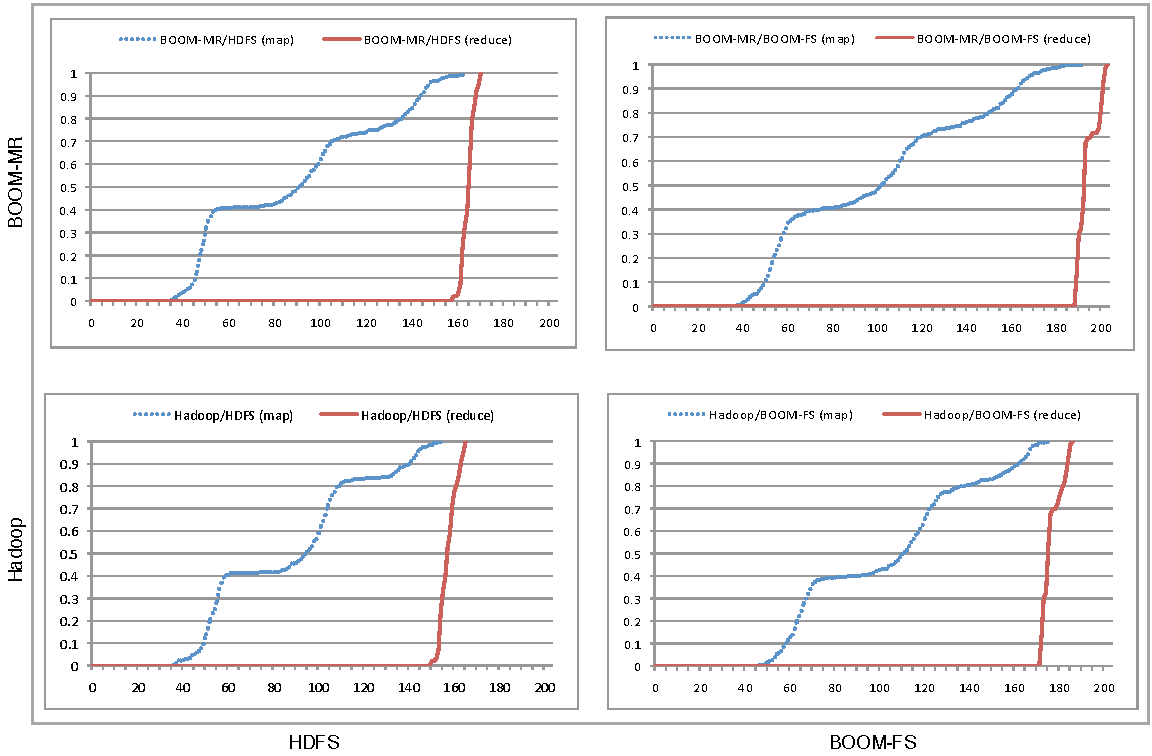
\includegraphics[scale=0.75]{figures/fourgraphs}
\caption{CDFs representing the elapsed time between job startup and task
  completion for both map and reduce tasks, for all combinations of Hadoop and \BOOM-MR
  over HDFS and \BOOM-FS\@.  In each graph, the horizontal axis is
  elapsed time in seconds, and the vertical represents the percentage of tasks completed.}
\label{fig:ec2experiment}
\end{figure*}

While improved performance was not a goal of our work, we wanted to
ensure that the performance of \BOOMA was competitive with Hadoop.
The workload was a wordcount job on a 30 GB file, using 481 map tasks 
and 100 reduce tasks.

Figure~\ref{fig:ec2experiment} contains four graphs comparing the performance of
different combinations of Hadoop MapReduce, HDFS, \BOOM-MR, and \BOOM-FS\@. Each
graph reports a cumulative distribution of the elapsed time in seconds from job
startup to map or reduce task completion. The map tasks complete in three
distinct ``waves.'' This is because only 2 $\times$ 100 map tasks can be
scheduled at once. Although all 100 reduce tasks can be scheduled immediately,
no reduce task can finish until all maps have been completed because each reduce
task requires the output of all map tasks.

The lower-left graph describes the performance of Hadoop running on top of HDFS,
and hence serves as a baseline for the subsequent graphs. The upper-left graph
details \BOOM-MR running over HDFS\@. This graph shows that map and reduce task
durations under \BOOM-MR are nearly identical to Hadoop 18.1. The lower-right
and upper-right graphs detail the performance of Hadoop MapReduce and \BOOM-MR
running on top of \BOOM-FS, respectively. \BOOM-FS performance is slightly
slower than HDFS, but remains competitive.


\subsection{LATE Evaluation}

\begin{figure*}
\ssp
  \centering
  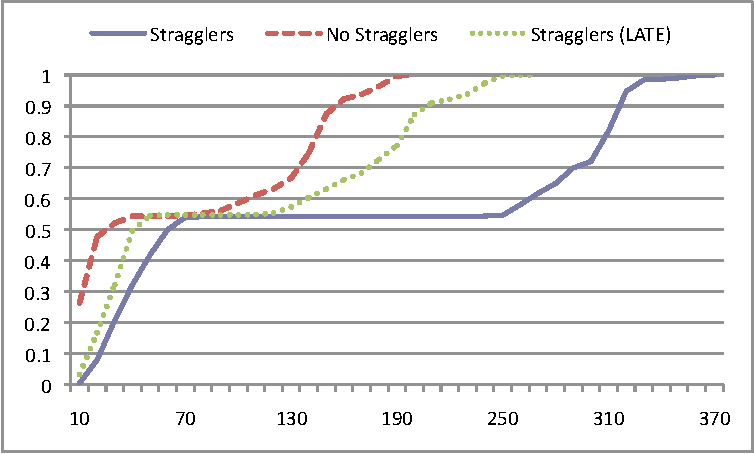
\includegraphics{figures/reduce_stragglers}
  \caption{CDF of reduce task duration (secs), with and without stragglers.}
  \label{fig:ec2reduce}
\end{figure*}

We now compare the behavior of our LATE implementation with the results observed
by Zaharia et al.\ using Hadoop MapReduce. LATE focuses on how to improve job completion time by reducing the impact of
``straggler'' tasks. To simulate stragglers, we artificially placed additional
load on six nodes. We ran a wordcount job on 30 GB of data, using 481 map tasks
and 400 reduce tasks (which produced two distinct ``waves'' of reduces). We ran
each experiment five times, and report the average over all
runs. Figure~\ref{fig:ec2reduce} shows the reduce task duration CDF for three
different configurations. The plot labeled ``No Stragglers'' represents normal
load, while the ``Stragglers'' and ``Stragglers (LATE)'' plots describe
performance in the presence in stragglers using the default FCFS policy and the
LATE policy, respectively. We omit map task durations, because adding artificial
load had little effect on map task execution --- it just resulted in slightly
slower growth from just below 100\% to completion.

The first wave of 200 reduce tasks was scheduled at the beginning of the
job. This first wave of reduce tasks cannot finish until all map tasks have
completed, which increased the duration of these tasks as indicated in the right
portion of the graph. The second wave of 200 reduce tasks did not experience
delay due to unfinished map work since it was scheduled after all map tasks had
finished. These shorter task durations are reported in the left portion of the
graph. Furthermore, stragglers had less impact on the second wave of reduce
tasks since less work (i.e., no map work) is being
performed. Figure~\ref{fig:ec2reduce} shows this effect, and also demonstrates
how the LATE implementation in {\BOOMA} handles stragglers much more effectively
than the FCFS policy ported from Hadoop.  This echoes the results of Zaharia et
al.~\cite{late-sched}



\section{Conclusion}
The initial version of \BOOM-MR required one person-month of
development time. We spent an additional two person-months debugging
and tuning \BOOM-MR's performance for large jobs. At the present time, 
\BOOM-MR represents the declarative specification of the core task scheduler (9 rules), 
the speculative task scheduler (5 rules), recovery from failed tasks (3 rules), and maintaining various 
job and task statistics (5 rules). In total, \BOOM-MR consists of 22 Overlog rules in 156 lines of 
code, and 1269 lines of Java. \BOOM-MR is based on Hadoop version 18.1; we estimate 
that we removed 6,573 lines from Hadoop (out of 88,864). The removed code contained
the core scheduling logic and the data structures that represent the
components listed in Table~\ref{tbl:hcatalog}. The Overlog patch that
replaces the original Hadoop scheduler contains an order of magnitude
fewer lines of code.  The performance of \BOOM-MR is very similar to
that of Hadoop MapReduce, as we discuss in Section~\ref{ch:boom:sec:eval}.

%% Our experience gutting Hadoop and inserting \BOOMA was not always
%% pleasant.  Given that we were committed to preserving the client API,
%% we did not take a ``purist'' approach and try to convert everything
%% into tables and Overlog rules.  For example, we chose not to
%% ``tableize'' the JobConf object, but instead to carry it through
%% Overlog tuples.  In our Overlog rules, we pass the JobConf object into
%% a custom Java table function that manufactures {\em task} tuples for
%% the job, subject to the specifications in the JobConf.

For this ``porting'' exercise, it was handy to leverage \JOL's Java interfaces
and draw the Java/Overlog boundaries flexibly.  This allowed us to focus on
porting the more interesting Hadoop logic into Overlog, while avoiding ports of
relatively mechanical details.  For example, we chose to leave the data
representation of the \emph{jobConf} as a Java object rather than flatten it
into a relation because it had no effect on the scheduling logic.

We found that scheduling policies were a good fit for a declarative language
like Overlog. In retrospect, this is because scheduling can be decomposed into
two tasks: \emph{monitoring} the state of a system and applying \emph{policies}
for how to react to changes to that state. Monitoring is well-handled by
Overlog: we found that the statistics about {\TT} state required by the LATE
policy are naturally realized as aggregate functions, and \JOL took care of
automatically updating those statistics as new messages from {\TT}s arrived. It
is also unsurprisingly that a logic language should be well-suited to specifying
policy. Overall, we found the \BOOM-MR scheduler much simpler to extend and
modify than the original Hadoop Java code, as demonstrated by our experience
with LATE\@.  Informally, the Overlog code in \BOOM-MR seems about as complex as
it should be: Hadoop's MapReduce task coordination logic is a simple and clean
design, and the compactness of \BOOM-MR reflects that simplicity appropriately.

